\documentclass[11pt,a4paper]{article}
\usepackage[utf8]{inputenc}
\usepackage[T1]{fontenc}
\usepackage[turkish]{babel}
\usepackage{lmodern}
\usepackage{microtype}
\usepackage{amsmath, amssymb, amsfonts}
\usepackage[margin=2.4cm]{geometry}
\usepackage{setspace}
\usepackage{url}
\usepackage{xurl}
\usepackage{booktabs}
\usepackage{tabularx}
\usepackage{graphicx}
\onehalfspacing

\title{\textbf{L2: Kaynak Yoksa Uyum da Yoktur --- Model Destekli Fizikte Literatür\\
Değerleri İçin Adli Protokol}}
\author{Fahri Meral}
\date{20 Ekim 2026}

\begin{document}
\shorthandoff{=}

\maketitle

\begin{abstract}
Kendi yayımlanmış ön-baskı serimizdeki, kendi kaynaklığımızdan gelen bir hatayı
ve onu aktarılabilir bir yönteme dönüştürüyoruz. Bir viskoelastik girdap
deneyi için ölçümsel oranlar tablosu \emph{bağımsız literatür, model dışı}
 olarak etiketlenmiş ve iki model çıktısıyla karşılaştırılmıştı. İki model
çıktısı iki alıntılanan aralığın içine düşüyordu. Aralıkların daha sonra
hiçbir kaynakta bulunmadığı gösterildi: dört birincil makale tam olarak
indirildi ve tarandı (PDF metni \emph{ve} LaTeX kaynağı) ve alıntılanan
sayılar onların hiçbirinde geçmiyor. İddia geri çekildi. İki bağımsız adli
test tanıtıldı ve kod olarak yayımlandı: \emph{depo arkeolojisi}, bir
değerin onu kullanan uyum iddiası \emph{öncesinde} hiçbir zaman kaynak kaydı
taşıyıp taşımadığını sorar; \emph{kaynak varlık taraması} ise alıntılanan
aralığın kaynak korpusunda hiç var olup olmadığını sorar. İki görünür teyidin
cebire bağımlı olduğunu gösteriyoruz --- ikinci oran, birincinin karesinin
kilitli bir sabite bölümüdür --- yani görünür iki noktalı uyum, kaynağı
olmayan tek bir serbestlik derecesine dayanıyordu. Etkilenen iki testte
kullanılan altı literatür büyüklüğünden üçü hiçbir kaynağa izlenemiyordu ve
ikisi daha sayısal olarak yanlıştı. Altı adımlık tespit protokolünü
veriyor, iki testin neyi, neyi belirleyemediğini açıkça söylüyor ve aracı,
bağımsız kendi kendini denetimini (7/7) ve adli figürü yayımlıyoruz.
\end{abstract}

\section{Sorun: aralıklar en tehlikeli artifacttır}
Bir model çıktısı literatür değeriyle karşılaştırıldığında doğal iki kontrol
şunlardır: \emph{doğru mu?} ve \emph{uyuyor mu?}. Hiçbiri, literatürde hiç
olmamış bir değeri tespit edemez. Yanlış bir nokta değeri, kaynağı bir kez
açtığınız anda yakalanır; hiç var olmayan bir \emph{aralık} ise yalnızca
kaynağı tüketerek yakalanabilir — bu pahalıdır ve, yanlış bir sayının
tersine, hiçbir hata imzası yoktur.

Aralıkları bu arızaya özellikle yatkın kılan üç özellik vardır.
\begin{enumerate}
    \item \emph{Uydurması ucuz, yanlışlanması pahalıdır.} İki yuvarlak sayı
    bir ölçüm özeti gibi görünür. ``$r \in [1.55,1.70]$'' ifadesi, bir
    şekil ekseni özetine tıpatıp benzer.
    \item \emph{Kendini mühürler.} Bir model değeri aralığın içine düşerse,
    uyum değeri doğruluyor gibi görünür — ve değer de modeli doğruluyor
    gibi görünür. Hiçbir dış kontrol tetiklenmez.
    \item \emph{Çürütme asimetrisini atlatır.} Yanlış bir nokta değeri yanlış
    bir öngörüye yol açar. Hayalet bir aralık ise yanlış bir \emph{teyide}
    yol açar; bu daha kötüdür, çünkü hiçbir sonraki hesapta görünmez.
\end{enumerate}
Bu mektup, tam olarak bu arızanın, kendi çalışmamızda, bir vaka çalışmasıdır;
yöntem ve yayımlanan araç ile birlikte.

\section{Vaka}
Daha sonra SS-XIV olarak numaralandırılan ön-baskı serisinde, T35 testi iki
disklu tankta 100\,ppm poliakrilamit oksit çözeltisi için öngörülen boyutsuz
oranları iki alıntılanan aralıkla karşılaştırdı,
\begin{equation}
\label{eq:bands}
r_{\mathrm{PEO}}/r_{\mathrm{su}} \in [1.55,\,1.70],
\qquad
\Delta h_{\mathrm{PEO}}/\Delta h_{\mathrm{su}} \in [0.30,\,0.35],
\end{equation}
ve bunları \emph{bağımsız literatür (model dışı)} olarak etiketledi. Model
çıktıları ise
\begin{equation}
\label{eq:model}
r_{\mathrm{PEO}}/r_{\mathrm{su}} = 1.626037936551738,
\qquad
\Delta h_{\mathrm{PEO}}/\Delta h_{\mathrm{su}} = 0.314025361279003
\end{equation}
idi; Denk.~\eqref{eq:model} her iki durumda da Denk.~\eqref{eq:bands} içindedir
--- aralıklar teyit olarak okundu.

\subsection{Aralıkların kökeni}
\begin{itemize}
    \item Alıntılanan aralıklar, uyumu ileri süren \emph{aynı} commit'te
    zaten \emph{bağımsız literatür} çerçevesinde depoya girdi
    (\texttt{043f2ee}, 19 Ekim 2026, 20:14).
    \item 56 dakika sonra (commit \texttt{96467dd}, 21:10) kaynak denetimi
    dört birincil makaleyi indirdi ve tam olarak taradı: Groisman \& Steinberg
    (2000) \cite{gs2000}; van Buel \& Stark (2022) \cite{vbs2022}; Guido vd.\
    (2021) \cite{guido2021}; Burghelea vd.\ (2006) \cite{bss2006}.
    \item Groisman \& Steinberg'in LaTeX kaynağında \texttt{1.55},
    \texttt{1.70}, \texttt{0.30}, \texttt{0.35}, \emph{funnel},
    \emph{dimple}, \emph{core} ve \emph{free surface} dizeleri hiç geçmez;
    çıkarılan PDF metninde (19\,519 karakter) ne \texttt{1.55} ne
    \texttt{1.70} vardır. Söz konusu deney, iki paralel disk arasında
    poliakrilamit + şuruptur, $d/R = 0.263$'tir ve şekil envanteri (şema;
    $\sigma/\sigma_{\rm lam}$ -- $\dot\gamma$; snapshot'lar; iki Fourier
    spektrumu) hiçbir serbest yüzey ya da dimple ölçümü içermez.
    \item Dolayısıyla aralıklar geri çekildi ve karşılaştırma kaldırıldı.
\end{itemize}
Altta yatan fizik gerçektir ve kaynaklanabilirdir --- aynı literatür, 10 ve
20\,mm aralıklar için $\sigma/\sigma_{\rm lam} = 12$ ve $19$ akış direnci
artışı, $\mathrm{Wi}_c = 12$ kritik Weissenberg sayısı ve elastik
türbülansın yeni uzunluk ölçeği olarak sınır tabakası kalınlığını
bildirmektedir --- ama alıntılanan aralık çifti hiçbir şeye izlenebilir
değildir.

\section{İki adli test}
\subsection{Depo arkeolojisi}
İlk test literatürde değeri aramaz; onu projenin kendi tarihinde arar. Bir
kaynaktan aktarılmış literatür değeri, model çıktısıyla karşılaştırılmadan
önce bir noktada \emph{literatür değeri olarak} yazılmış olmalıdır. Bu
yüzden commit tarihçesindeki üç ilk görünüşü karşılaştırıyoruz:
\begin{align}
t_{\mathrm{ilk}} &:\ \text{jetonun ilk bağımsız görünüşü},\\
t_{\mathrm{ref}} &:\ \text{referans çerçevesindeki ilk görünüş},\\
t_{\mathrm{iddia}} &:\ \text{uyum iddiasındaki ilk görünüş}.
\end{align}
Eğer $t_{\mathrm{ref}} = t_{\mathrm{iddia}}$ ise değer bir uyum olarak doğmuş
demektir: onu kaynaklı bir veri olarak gösteren daha önce bir kayıt yoktur ve
\emph{bağımsız literatür} etiketi iddianın anında uygulanmış, bir kaynaktan
türetilmiş değildir.

İki uygulama ayrıntısı önemlidir ve yayımlanan araçta zorlanır. Birincisi,
arama \emph{bağımsız jeton} için olmalıdır: \texttt{1.55} için alt dize
araması, projenin ilk commit'indeki alakasız \texttt{1.556152e+05}
büyüklüğünü bulur ve sahte bir köken kaydı üretir. İkincisi, referans ve
iddia çerçeveleri $\pm3$ satırlık pencerede saptanır, çünkü atıf ile onun
sayısı rutin olarak iki satıra bölünür.

\subsection{Kaynak varlık taraması}
İkinci test, alıntılanan aralığın kaynak korpusunda hiç var olup olmadığını
sorar: korpustaki her arXiv LaTeX kaynağı ve her PDF, jeton sınırlarıyla
taranır ve bir aralığın üyelerinin birlikte bulunduğu dosya sayısı ayrıca
bildirilir. Tarama başarısızlıkları açıkça raporlamak zorundadır; metni
çıkarılamayan bir PDF asla sıfır sayılmaz, hata sayılır.

T35 ve T36'da kullanılan literatür değerleri için korpus (100 dosya: 81 PDF
— bunların 17'si birincil makaleler — ve 19 arXiv LaTeX kaynak dosyası)
sonuçları:
\begin{table}[!htbp]
\centering\footnotesize
\setlength{\tabcolsep}{5pt}
\caption{\textbf{T35 ve T36'da kullanılan literatür değerlerinin varlık
taraması.} Korpus: 100 dosya (81 PDF + 19 arXiv LaTeX kaynağı). Eşleşmeler
jeton sınırlarıyla sayılır. \emph{Eş-şidd}, bir aralığın üyelerinin birlikte
bulunduğu dosya sayısıdır.}
\label{tab:scan}
\vspace{0.1cm}
\begin{tabular}{@{}llrr@{}}
\toprule
Değer & Depo kararı & Eşleşme & Eş-şidd \\
\midrule
\texttt{1.55} & GHOST\_CANDIDATE & 0 & --- \\
\texttt{1.70} & GHOST\_CANDIDATE & 0 & --- \\
\texttt{1.55\,+\,1.70} (aralık) & GHOST\_CANDIDATE & 0 & 0 \\
\texttt{0.30} & GHOST\_CANDIDATE & 4 & --- \\
\texttt{0.35} & HAS\_PROVENANCE & 5 & --- \\
\texttt{0.30\,+\,0.35} (aralık) & GHOST\_CANDIDATE & 9 & 3 \\
\texttt{2.25} (glitch bandı) & GHOST\_CANDIDATE & 2 & --- \\
\texttt{0.0160} ($I_{\rm crust}/I$) & GHOST\_CANDIDATE & 0 & --- \\
\texttt{0.014} ($I_{\rm crust}/I$, düzeltilmiş) & GHOST\_CANDIDATE & 4 & --- \\
\bottomrule
\end{tabular}
\end{table}

Tablo~\ref{tab:scan}, bu mektubun bütün dersini iki satırda taşır.
\texttt{1.55} ve \texttt{1.70} hiçbir yerde geçmez, dolayısıyla aralık
hayalettir. Ama \texttt{0.30} ve \texttt{0.35} \emph{geçer}: dört ve beş
kez, ve üç dosyada birlikte --- bir 511\,keV çizgi modelleme makalesi, bir
ant hidrojen hiperfine makalesi ve iki INTEGRAL akış haritası --- viskoelastik
girdaplarla hiçbir ilgisi olmayan bağlamlarda. \emph{Jetonun varlığı
provenance değildir; bağlam olmadan eş-şidd de provenance değildir.} Yalnız
kaynağın anlamsal okunuşu bunu kapatır; bu yüzden en ucuz otomatikleştirilebilir
test --- arkeoloji --- iddia hâlâ geri çekilmesi ucuzken önce çalıştırılmalıdır.

\subsection{İki görünür teyit aslında bir taneydi}
Denk.~\eqref{eq:bands}'teki iki uyum cebire bağımlıdır. $a \equiv
\mathcal{C}_{\mathrm{univ}}$ ve kilitli $\mu_s$ ile
\begin{equation}
\label{eq:dep}
\frac{\Delta h_{\mathrm{PEO}}}{\Delta h_{\mathrm{su}}}
= \frac{1}{a^{2}(1+\mu_s)}
= \left(\frac{u_{\max}^{\mathrm{PEO}}}{u_{\max}^{\mathrm{su}}}\right)^{2}
\frac{1}{1+\mu_s},
\end{equation}
çünkü serbest yüzey çökmesi Burgers çekirdek yarıçapının karesiyle ters
oranlıdır, $r_c \propto a$. Sayısal olarak Denk.~\eqref{eq:dep} eşitliği
$5.6\times10^{-17}$ hassasiyetle, $r_{\mathrm{PEO}}/r_{\mathrm{su}} =
\mathcal{C}_{\mathrm{univ}}$ ise $2.2\times10^{-16}$ ile sağlanır. Dolayısıyla
ikinci aralık uyumu birincinin yeniden parametrelendirmesidir, onun bağımsız
bir testi değil: ikili tek bir serbestlik derecesine dayanır. Aralıkların
hayalet olmasıyla birleştiğinde, görünür iki noktalı teyit sıfıra çöker.

\section{Protokol}
Altı adım; bunlardan yalnız ilk üçü çoğu yazar için yeni pratiktir.
\begin{enumerate}
    \item \textbf{Her literatür değeri için kaynak satırı alıntılayın.}
    Dosya, tablo ya da şekil numarası ve sayfa. Konumu bulunabilir
    olmayan ``literatür'' alıntı değildir.
    \item \textbf{Kaynağın onu \emph{ içerdiğini} sorun.} Soru varlıktır,
    eşitlik değil. Bir aralık için, her iki üyenin birlikte, aynı bağlamda
    görünüp görünmediğini sorun.
    \item \textbf{Makine-okunur kaynağı tarayın.} arXiv makalelerinde
    LaTeX kaynağı, PDF metin çıkarımının kaçırdığı şekil altyazılarını,
    tablo notlarını ve ek malzemeyi bulur ve taramayı yeniden-üretilebilir
    kılar.
    \item \textbf{İlk görünüşü kurtarın.} Sürüm denetimli bir proje her
    değerin ne zaman ve hangi çerçevede girdiğine dair zaman damgalı bir
    kayıt tutar. Arama jeton sınırlarına uymalıdır.
    \item \textbf{Sıralamayı sınayın.} Bağımsız denen bir değer, onu kullanan
    uyum iddiasından \emph{önce} kaynaklı olarak kaydedilmiş olmalıdır. İlk
    referans ile ilk iddia aynı commit ise bağımsızlık türetilmiş değil,
    ileri sürülmüştür.
    \item \textbf{Onarmak yerine geri çekin.} Sayı izlenemiyorsa, onu
    kullanan iddia, fizik hayatta kalsa bile geri çekilir. Onu \emph{gerçekten}
    kaynaklanabilir değerle değiştirin ve geri çekilişi kayda geçirin.
\end{enumerate}
Adım 6 pahalı olanıdır ve adım 1'i ucuz kılan da odur: bir geri çekme bir
paragrafa mal olur; izlenemeyen bir teyit ise okuyucunun tablodaki geri kalan
satırlara güvenme yetisine mal olur.

\section{İki test neyi, neyi belirleyebilir}
Sınırları açıkça söylüyoruz, çünkü erişimini abartan bir adli araç bir sonraki
hayaletin kendisi olur.
\begin{itemize}
    \item \emph{Arkeoloji testi doğruluk hakkında hiçbir şey söylemez.}
    Bir değerin, onu kullanan iddiadan \emph{önce} \emph{bu} depoda kaynak
    kaydı taşıyıp taşımadığını bildirir. Düzeltilmiş kabuk oranı değeri
    $\Delta I/I \ge 0.014$ gerçekten kaynaklıdır (Link vd.~\cite{link1999}
    LaTeX kaynağında geçer) ve yine de işaretlenir; çünkü denetimden önce
    repo bu kaynağı hiç aktarmamıştı. İşaret bir kaynak satırı talebidir,
    bir çürütme değil.
    \item \emph{Depo kökeni belirleyemez.} Yalnızca provenance kaydının
    bulunmadığını belirler. Aralığın yanlış hatırlanmış mı, daha önceki bir
    çalışma notundan mı taşınmış, taslak sırasında bir dil modeli tarafından
    mı önerilmiş, yoksa bir hesap hatası mı olduğu depodan belirlenemez ve
    biz bunu iddia etmiyoruz.
    \item \emph{Varlık taraması basılı kaydı sınırlar, fiziği değil.} Sıfır
    eşleşme, alıntılanan sayıların taranan korpusta hiç geçmediğini
    gösterir; benzer bir ölçümün hiç yapılmadığını kanıtlamaz. Gösterdiği
    şey, yazıldığı haliyle iddianın geri getirilebilir bir temeli
    olmadığıdır.
\end{itemize}

\section{Bir test çiftinde sorunun ölçeği}
T35 ve T36 denetimleri altı literatür büyüklüğü kullandı: iki aralık, glitch
genliği $(2.25\pm0.35)\times10^{-6}$, iyileşme kesri $Q\in[0.05,0.18]$,
kabuk oranı $I_{\rm crust}/I$ ve glitch gevşeme zaman ölçekleri. Üçü hiçbir
kaynağa izlenemedi; ikisi daha sayısal olarak yanlıştı ve ölçülen değerlerle
değiştirildi ($I_{\rm crust}/I = 0.0160 \rightarrow \ge 0.014$, Link vd.\
kaynağından; keyfî 6 ve 60 günlük gevşeme süreleri $\rightarrow$ Dodson vd.\
\cite{dodson2002}'den ölçülen 1,2 dk, 0,53, 3,29 ve 19,07 gün); yalnız altıncısı
zaten doğruydu. \textbf{Altısından beşi düzeltme gerektirdi.} Bu seride oran
ancak kaynaklar sonunda indirilip okunduğunda sıfıra düştü.

\section{Yeniden-üretilebilirlik}
Tüm adli makine bu mektupla birlikte yayımlanmıştır:
\begin{itemize}
    \item \texttt{ghost\_audit.py} --- iki test: depo arkeolojisi (ilk
    görünüş, referans çerçevesi, iddia çerçevesi; jeton sınırlarının
    zorlanması ve $\pm3$ satırlık bağlam penceresi) ve kaynak varlık taraması
    (açık eş-şidd sayımı ve açık hata bildirimiyle).
    \item \texttt{mini\_check\_l2.py} --- bağımsız kendi denetimi: sentetik
    depolar ve korpuslar kurar, dört kararı
    (\texttt{GHOST\_CANDIDATE}, \texttt{HAS\_PROVENANCE},
    \texttt{NOT\_A\_LIT\_VALUE}, \texttt{ABSENT}), jeton sınırı kuralını,
    eş-şidd sayımını ve gerçek vakayı sınar: 7/7 PASS.
    \item Şekil 1 --- hayalet aralığın yaşam döngüsü, varlık taraması, iki
    görünür teyidin cebire çöküşü ve protokol.
\end{itemize}
Araç çözücüyü import etmez ve fiziksel modele bağlı değildir; bir depo ve bir
korpus üzerinde çalışır. Çalıştırma talimatları ek depodaki README dosyasındadır.

\clearpage
\begin{figure}[!htbp]
\centering
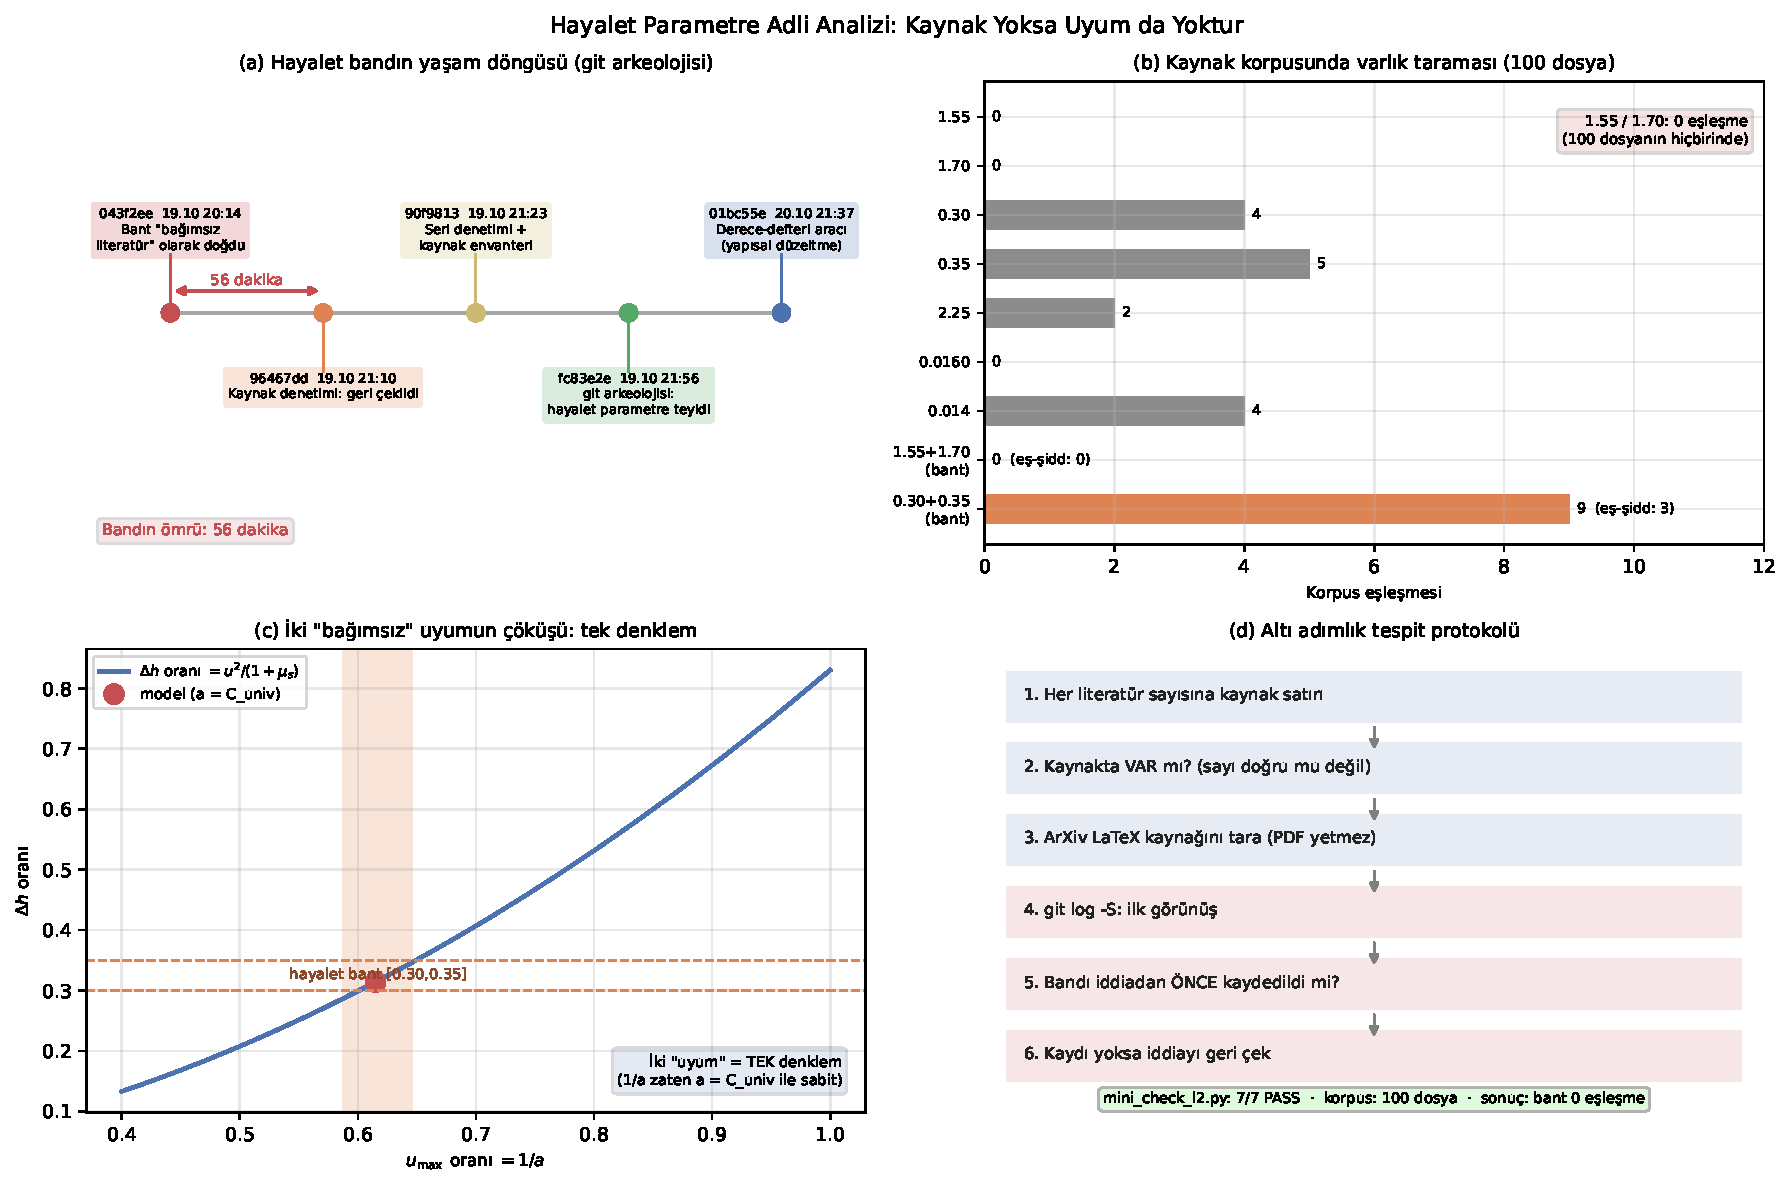
\includegraphics[width=\textwidth]{../figs/fig16_ghost_parameter_forensics.pdf}
\caption{\textbf{Hayalet aralığın adli özeti.}
(a) Aralık, commit \texttt{043f2ee}'de \emph{bağımsız literatür} olarak
doğdu ve 56 dakika sonra kaynak denetimi tarafından geri çekildi; arkeoloji
teyidi ve yapısal düzeltme (derece-defteri) ardından geldi. (b) Kaynak
korpusunda varlık taraması: \texttt{1.55} ve \texttt{1.70} hiçbir yerde
geçmiyor; \texttt{0.30} ve \texttt{0.35} geçiyor ve üç dosyada birlikte
geçiyor, ama alakasız bağlamlarda. (c) İki görünür teyit tek denklemdir:
çökme oranı, hız oranının karesinin $1+\mu_s$'e bölümüdür. (d) Altı adımlık
protokol.}
\label{fig:ghost}
\end{figure}

\clearpage
\begin{thebibliography}{99}
    \bibitem{gs2000} Groisman, A. A. \& Steinberg, V. (2000). Elastic
    turbulence in a polymer solution. \textit{Nature \textbf{405}}, 53--61.
    arXiv:nlin/0104052.
    \bibitem{vbs2022} van Buel, J. \& Stark, P. D. (2022). Elastic turbulence
    in dilute polymer solutions. arXiv:2202.12714.
    \bibitem{guido2021} Guido, S. \textit{et al.} (2021). Development of
    vortex based on polymeric solution. arXiv:2110.03004.
    \bibitem{bss2006} Burghelea, A., Segre, D. \& Steinberg, V. (2006).
    Elastic turbulence in a dilute polymer solution.
    arXiv:physics/0609112.
    \bibitem{link1999} Link, F., Epstein, D. L. \& Lattimer, J. M. (1999).
    Glitching pulsars. \textit{Phys.\ Rev.\ Lett.\ \textbf{83}}, 3807--3810.
    \bibitem{dodson2002} Dodson, R. N. \textit{et al.} (2002). Frequency
    behaviour of the Vela pulsar during the glitch of 2000 January.
    \textit{Astrophys.\ J.\ \textbf{574}}, 471--475.
    arXiv:astro-ph/0201005.
\end{thebibliography}

\end{document}
